\documentclass{standalone}
\usepackage{tikz}
\usetikzlibrary{patterns, positioning}
\usepackage[sfdefault]{ClearSans} %% option 'sfdefault' activates Clear Sans as the default text font
\usepackage[T1]{fontenc}

\begin{document}
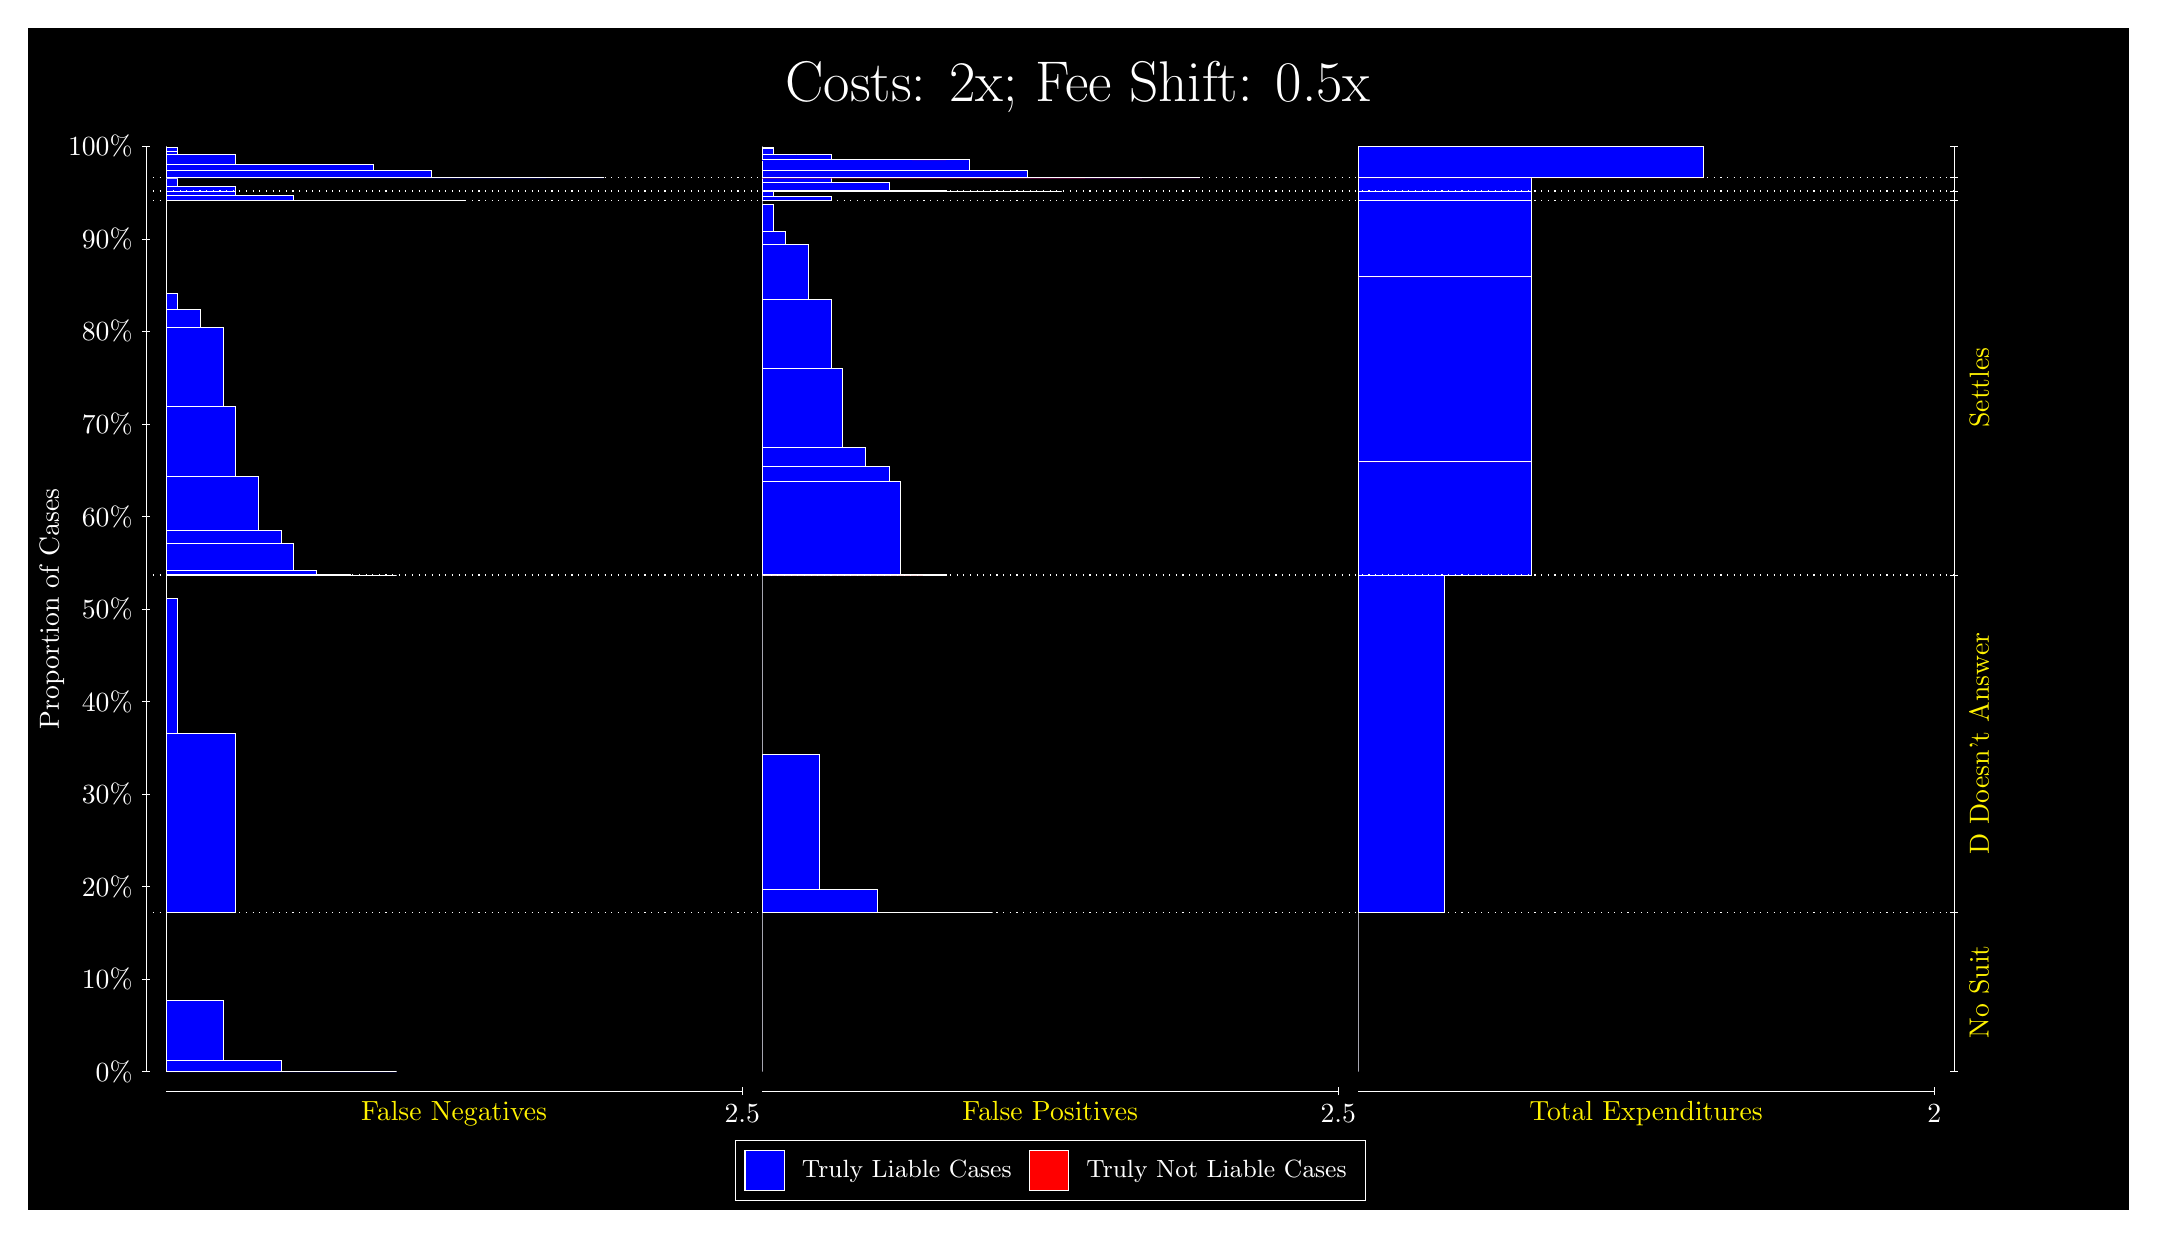
\begin{tikzpicture}
\draw[fill=black] (0,0) rectangle (26.667,15);
\draw[text=white] (0,13.5) rectangle (26.667,15) node[midway] {\huge Costs: 2x; Fee Shift: 0.5x};
\draw[white, very thin] (1.5,1.75) -- (1.5,13.5);
\node[rotate=90, text=white, anchor=center] at (0.3, 7.625) {Proportion of Cases};
\draw[white, very thin] (1.45,1.75) -- (1.55,1.75);
\node[text=white, anchor=east] at (1.45, 1.75) {0\%};
\draw[white, very thin] (1.45,2.925) -- (1.55,2.925);
\node[text=white, anchor=east] at (1.45, 2.925) {10\%};
\draw[white, very thin] (1.45,4.1) -- (1.55,4.1);
\node[text=white, anchor=east] at (1.45, 4.1) {20\%};
\draw[white, very thin] (1.45,5.275) -- (1.55,5.275);
\node[text=white, anchor=east] at (1.45, 5.275) {30\%};
\draw[white, very thin] (1.45,6.45) -- (1.55,6.45);
\node[text=white, anchor=east] at (1.45, 6.45) {40\%};
\draw[white, very thin] (1.45,7.625) -- (1.55,7.625);
\node[text=white, anchor=east] at (1.45, 7.625) {50\%};
\draw[white, very thin] (1.45,8.8) -- (1.55,8.8);
\node[text=white, anchor=east] at (1.45, 8.8) {60\%};
\draw[white, very thin] (1.45,9.975) -- (1.55,9.975);
\node[text=white, anchor=east] at (1.45, 9.975) {70\%};
\draw[white, very thin] (1.45,11.15) -- (1.55,11.15);
\node[text=white, anchor=east] at (1.45, 11.15) {80\%};
\draw[white, very thin] (1.45,12.325) -- (1.55,12.325);
\node[text=white, anchor=east] at (1.45, 12.325) {90\%};
\draw[white, very thin] (1.45,13.5) -- (1.55,13.5);
\node[text=white, anchor=east] at (1.45, 13.5) {100\%};

\draw[white, very thin] (24.457,1.75) -- (24.457,13.5);
\draw[white, very thin] (24.407,1.75) -- (24.507,1.75);
\node[anchor=west] at (24.407, 1.75) {};
\draw[white, very thin] (24.407,3.7706) -- (24.507,3.7706);
\node[anchor=west] at (24.407, 3.7706) {};
\draw[white, very thin] (24.407,8.0563) -- (24.507,8.0563);
\node[anchor=west] at (24.407, 8.0563) {};
\draw[white, very thin] (24.407,12.817) -- (24.507,12.817);
\node[anchor=west] at (24.407, 12.817) {};
\draw[white, very thin] (24.407,12.933) -- (24.507,12.933);
\node[anchor=west] at (24.407, 12.933) {};
\draw[white, very thin] (24.407,13.102) -- (24.507,13.102);
\node[anchor=west] at (24.407, 13.102) {};
\draw[white, very thin] (24.407,13.5) -- (24.507,13.5);
\node[anchor=west] at (24.407, 13.5) {};

\draw[white, very thin, fill=blue] (1.75,1.75) rectangle (4.6775,1.75);
\draw[white, very thin, fill=blue] (1.75,1.75) rectangle (3.9457,1.7512);
\draw[white, very thin, fill=blue] (1.75,1.7512) rectangle (3.2138,1.8873);
\draw[white, very thin, fill=blue] (1.75,1.8873) rectangle (2.4819,2.6572);
\draw[white, very thin, fill=red] (1.75,2.6572) rectangle (1.75,2.6572);
\draw[white, very thin, fill=blue] (1.75,2.6572) rectangle (1.75,3.7706);
\draw[white, very thin, fill=blue] (1.75,3.7706) rectangle (2.6283,6.0452);
\draw[white, very thin, fill=blue] (1.75,6.0452) rectangle (1.8964,7.7596);
\draw[white, very thin, fill=red] (1.75,7.7596) rectangle (1.75,7.7596);
\draw[white, very thin, fill=blue] (1.75,7.7596) rectangle (1.75,8.0563);
\draw[white, very thin, fill=blue] (1.75,8.0563) rectangle (4.6775,8.0563);
\draw[white, very thin, fill=blue] (1.75,8.0563) rectangle (4.3848,8.0563);
\draw[white, very thin, fill=blue] (1.75,8.0563) rectangle (4.092,8.066);
\draw[white, very thin, fill=blue] (1.75,8.066) rectangle (3.9457,8.0667);
\draw[white, very thin, fill=blue] (1.75,8.0667) rectangle (3.6529,8.1133);
\draw[white, very thin, fill=blue] (1.75,8.1133) rectangle (3.3602,8.4573);
\draw[white, very thin, fill=blue] (1.75,8.4573) rectangle (3.2138,8.6233);
\draw[white, very thin, fill=blue] (1.75,8.6233) rectangle (2.921,9.3125);
\draw[white, very thin, fill=blue] (1.75,9.3125) rectangle (2.6283,10.195);
\draw[white, very thin, fill=blue] (1.75,10.195) rectangle (2.4819,11.201);
\draw[white, very thin, fill=blue] (1.75,11.201) rectangle (2.1891,11.433);
\draw[white, very thin, fill=blue] (1.75,11.433) rectangle (1.8964,11.632);
\draw[white, very thin, fill=red] (1.75,11.632) rectangle (1.75,11.632);
\draw[white, very thin, fill=blue] (1.75,11.632) rectangle (1.75,12.817);
\draw[white, very thin, fill=blue] (1.75,12.817) rectangle (5.5558,12.817);
\draw[white, very thin, fill=blue] (1.75,12.817) rectangle (4.8239,12.817);
\draw[white, very thin, fill=blue] (1.75,12.817) rectangle (4.092,12.819);
\draw[white, very thin, fill=blue] (1.75,12.819) rectangle (3.3602,12.883);
\draw[white, very thin, fill=blue] (1.75,12.883) rectangle (2.6283,12.933);
\draw[white, very thin, fill=red] (1.75,12.933) rectangle (1.75,12.933);
\draw[white, very thin, fill=blue] (1.75,12.933) rectangle (2.6283,12.995);
\draw[white, very thin, fill=blue] (1.75,12.995) rectangle (1.8964,13.096);
\draw[white, very thin, fill=red] (1.75,13.096) rectangle (1.75,13.096);
\draw[white, very thin, fill=blue] (1.75,13.096) rectangle (1.75,13.102);
\draw[white, very thin, fill=blue] (1.75,13.102) rectangle (7.3123,13.102);
\draw[white, very thin, fill=blue] (1.75,13.102) rectangle (6.5805,13.102);
\draw[white, very thin, fill=blue] (1.75,13.102) rectangle (5.8486,13.109);
\draw[white, very thin, fill=blue] (1.75,13.109) rectangle (5.1167,13.2);
\draw[white, very thin, fill=blue] (1.75,13.2) rectangle (4.8239,13.2);
\draw[white, very thin, fill=blue] (1.75,13.2) rectangle (4.3848,13.27);
\draw[white, very thin, fill=blue] (1.75,13.27) rectangle (4.092,13.27);
\draw[white, very thin, fill=blue] (1.75,13.27) rectangle (3.6529,13.27);
\draw[white, very thin, fill=blue] (1.75,13.27) rectangle (3.3602,13.272);
\draw[white, very thin, fill=blue] (1.75,13.272) rectangle (2.921,13.272);
\draw[white, very thin, fill=blue] (1.75,13.272) rectangle (2.6283,13.274);
\draw[white, very thin, fill=blue] (1.75,13.274) rectangle (2.6283,13.402);
\draw[white, very thin, fill=blue] (1.75,13.402) rectangle (1.8964,13.436);
\draw[white, very thin, fill=blue] (1.75,13.436) rectangle (1.8964,13.494);
\draw[white, very thin, fill=red] (1.75,13.494) rectangle (1.75,13.494);
\draw[white, very thin, fill=blue] (1.75,13.494) rectangle (1.75,13.5);
\draw[white, very thin, fill=red] (9.3189,1.75) rectangle (9.3189,1.75);
\draw[white, very thin, fill=blue] (9.3189,1.75) rectangle (9.3189,3.7706);
\draw[white, very thin, fill=red] (9.3189,3.7706) rectangle (12.246,3.7706);
\draw[white, very thin, fill=blue] (9.3189,3.7706) rectangle (12.246,3.7706);
\draw[white, very thin, fill=blue] (9.3189,3.7706) rectangle (11.515,3.7724);
\draw[white, very thin, fill=blue] (9.3189,3.7724) rectangle (10.783,4.0673);
\draw[white, very thin, fill=blue] (9.3189,4.0673) rectangle (10.051,5.7816);
\draw[white, very thin, fill=blue] (9.3189,5.7816) rectangle (9.3189,8.0563);
\draw[white, very thin, fill=red] (9.3189,8.0563) rectangle (11.661,8.0563);
\draw[white, very thin, fill=blue] (9.3189,8.0563) rectangle (11.661,8.0612);
\draw[white, very thin, fill=red] (9.3189,8.0612) rectangle (11.368,8.0612);
\draw[white, very thin, fill=blue] (9.3189,8.0612) rectangle (11.368,8.066);
\draw[white, very thin, fill=red] (9.3189,8.066) rectangle (11.075,8.066);
\draw[white, very thin, fill=blue] (9.3189,8.066) rectangle (11.075,9.2416);
\draw[white, very thin, fill=blue] (9.3189,9.2416) rectangle (10.929,9.4406);
\draw[white, very thin, fill=blue] (9.3189,9.4406) rectangle (10.636,9.6727);
\draw[white, very thin, fill=blue] (9.3189,9.6727) rectangle (10.344,10.679);
\draw[white, very thin, fill=blue] (9.3189,10.679) rectangle (10.197,11.561);
\draw[white, very thin, fill=blue] (9.3189,11.561) rectangle (9.9044,12.25);
\draw[white, very thin, fill=blue] (9.3189,12.25) rectangle (9.6116,12.416);
\draw[white, very thin, fill=blue] (9.3189,12.416) rectangle (9.4652,12.76);
\draw[white, very thin, fill=blue] (9.3189,12.76) rectangle (9.3189,12.817);
\draw[white, very thin, fill=red] (9.3189,12.817) rectangle (10.197,12.817);
\draw[white, very thin, fill=blue] (9.3189,12.817) rectangle (10.197,12.867);
\draw[white, very thin, fill=blue] (9.3189,12.867) rectangle (9.4652,12.931);
\draw[white, very thin, fill=blue] (9.3189,12.931) rectangle (9.3189,12.933);
\draw[white, very thin, fill=red] (9.3189,12.933) rectangle (13.125,12.933);
\draw[white, very thin, fill=blue] (9.3189,12.933) rectangle (13.125,12.933);
\draw[white, very thin, fill=blue] (9.3189,12.933) rectangle (12.393,12.933);
\draw[white, very thin, fill=blue] (9.3189,12.933) rectangle (11.661,12.938);
\draw[white, very thin, fill=blue] (9.3189,12.938) rectangle (10.929,13.039);
\draw[white, very thin, fill=blue] (9.3189,13.039) rectangle (10.197,13.102);
\draw[white, very thin, fill=red] (9.3189,13.102) rectangle (14.881,13.102);
\draw[white, very thin, fill=blue] (9.3189,13.102) rectangle (14.881,13.102);
\draw[white, very thin, fill=red] (9.3189,13.102) rectangle (14.149,13.102);
\draw[white, very thin, fill=blue] (9.3189,13.102) rectangle (14.149,13.102);
\draw[white, very thin, fill=red] (9.3189,13.102) rectangle (13.417,13.102);
\draw[white, very thin, fill=blue] (9.3189,13.102) rectangle (13.417,13.107);
\draw[white, very thin, fill=red] (9.3189,13.107) rectangle (12.686,13.107);
\draw[white, very thin, fill=blue] (9.3189,13.107) rectangle (12.686,13.199);
\draw[white, very thin, fill=blue] (9.3189,13.199) rectangle (11.954,13.33);
\draw[white, very thin, fill=red] (9.3189,13.33) rectangle (11.661,13.33);
\draw[white, very thin, fill=blue] (9.3189,13.33) rectangle (11.661,13.33);
\draw[white, very thin, fill=blue] (9.3189,13.33) rectangle (11.222,13.331);
\draw[white, very thin, fill=red] (9.3189,13.331) rectangle (10.929,13.331);
\draw[white, very thin, fill=blue] (9.3189,13.331) rectangle (10.929,13.332);
\draw[white, very thin, fill=blue] (9.3189,13.332) rectangle (10.49,13.332);
\draw[white, very thin, fill=blue] (9.3189,13.332) rectangle (10.197,13.401);
\draw[white, very thin, fill=red] (9.3189,13.401) rectangle (10.197,13.401);
\draw[white, very thin, fill=blue] (9.3189,13.401) rectangle (10.197,13.402);
\draw[white, very thin, fill=blue] (9.3189,13.402) rectangle (9.758,13.402);
\draw[white, very thin, fill=blue] (9.3189,13.402) rectangle (9.4652,13.475);
\draw[white, very thin, fill=blue] (9.3189,13.475) rectangle (9.4652,13.493);
\draw[white, very thin, fill=blue] (9.3189,13.493) rectangle (9.3189,13.5);
\draw[white, very thin, fill=red] (16.888,1.75) rectangle (16.888,1.75);
\draw[white, very thin, fill=blue] (16.888,1.75) rectangle (16.888,3.7706);
\draw[white, very thin, fill=red] (16.888,3.7706) rectangle (17.986,3.7706);
\draw[white, very thin, fill=blue] (16.888,3.7706) rectangle (17.986,8.0563);
\draw[white, very thin, fill=red] (16.888,8.0563) rectangle (19.083,8.0563);
\draw[white, very thin, fill=blue] (16.888,8.0563) rectangle (19.083,9.4958);
\draw[white, very thin, fill=red] (16.888,9.4958) rectangle (19.083,9.4958);
\draw[white, very thin, fill=blue] (16.888,9.4958) rectangle (19.083,11.844);
\draw[white, very thin, fill=red] (16.888,11.844) rectangle (19.083,11.844);
\draw[white, very thin, fill=blue] (16.888,11.844) rectangle (19.083,12.817);
\draw[white, very thin, fill=red] (16.888,12.817) rectangle (19.083,12.817);
\draw[white, very thin, fill=blue] (16.888,12.817) rectangle (19.083,12.933);
\draw[white, very thin, fill=red] (16.888,12.933) rectangle (19.083,12.933);
\draw[white, very thin, fill=blue] (16.888,12.933) rectangle (19.083,13.102);
\draw[white, very thin, fill=red] (16.888,13.102) rectangle (21.279,13.102);
\draw[white, very thin, fill=blue] (16.888,13.102) rectangle (21.279,13.5);
\draw[white, dotted] (1.5,3.7706) -- (24.457,3.7706);
\draw[white, dotted] (1.5,8.0563) -- (24.457,8.0563);
\draw[white, dotted] (1.5,12.817) -- (24.457,12.817);
\draw[white, dotted] (1.5,12.933) -- (24.457,12.933);
\draw[white, dotted] (1.5,13.102) -- (24.457,13.102);
\draw[white, very thin] (1.75,1.5) -- (9.0689,1.5);
\node[text=yellow, anchor=north] at (5.4094, 1.5) {False Negatives};
\draw[white, very thin] (9.0689,1.45) -- (9.0689,1.55);
\node[text=white, anchor=north] at (9.0689, 1.45) {2.5};

\draw[white, very thin] (9.3189,1.5) -- (16.638,1.5);
\node[text=yellow, anchor=north] at (12.978, 1.5) {False Positives};
\draw[white, very thin] (16.638,1.45) -- (16.638,1.55);
\node[text=white, anchor=north] at (16.638, 1.45) {2.5};

\draw[white, very thin] (16.888,1.5) -- (24.207,1.5);
\node[text=yellow, anchor=north] at (20.547, 1.5) {Total Expenditures};
\draw[white, very thin] (24.207,1.45) -- (24.207,1.55);
\node[text=white, anchor=north] at (24.207, 1.45) {2};

\node[text=yellow, centered, rotate=90] at (24.777, 2.7603) {No Suit};
\node[text=yellow, centered, rotate=90] at (24.777, 5.9134) {D Doesn't Answer};
\node[text=yellow, centered, rotate=90] at (24.777, 10.437) {Settles};




\draw (12.978300999999998,1.5) node[draw=none] (baseCoordinate) {};
\begin{scope}[align=center]
        \matrix[scale=0.5, draw=white, below=0.5cm of baseCoordinate, nodes={draw}, column sep=0.1cm]{
            \node[rectangle, draw, minimum width=0.5cm, minimum height=0.5cm, fill=blue] {}; &
            \node[draw=none, font=\small, text=white] (B) {Truly Liable Cases}; &
            \node[rectangle, draw, minimum width=0.5cm, minimum height=0.5cm, fill=red] {}; &
            \node[draw=none, font=\small, text=white] (B) {Truly Not Liable Cases}; \\
            };
\end{scope}

\end{tikzpicture}
\end{document}